\documentclass[twoside]{book}

% Packages required by doxygen
\usepackage{calc}
\usepackage{doxygen}
\usepackage{graphicx}
\usepackage[utf8]{inputenc}
\usepackage{makeidx}
\usepackage{multicol}
\usepackage{multirow}
\usepackage{textcomp}
\usepackage[table]{xcolor}

% Font selection
\usepackage[T1]{fontenc}
\usepackage{mathptmx}
\usepackage[scaled=.90]{helvet}
\usepackage{courier}
\usepackage{amssymb}
\usepackage{sectsty}
\renewcommand{\familydefault}{\sfdefault}
\allsectionsfont{%
  \fontseries{bc}\selectfont%
  \color{darkgray}%
}
\renewcommand{\DoxyLabelFont}{%
  \fontseries{bc}\selectfont%
  \color{darkgray}%
}

% Page & text layout
\usepackage{geometry}
\geometry{%
  a4paper,%
  top=2.5cm,%
  bottom=2.5cm,%
  left=2.5cm,%
  right=2.5cm%
}
\tolerance=750
\hfuzz=15pt
\hbadness=750
\setlength{\emergencystretch}{15pt}
\setlength{\parindent}{0cm}
\setlength{\parskip}{0.2cm}
\makeatletter
\renewcommand{\paragraph}{%
  \@startsection{paragraph}{4}{0ex}{-1.0ex}{1.0ex}{%
    \normalfont\normalsize\bfseries\SS@parafont%
  }%
}
\renewcommand{\subparagraph}{%
  \@startsection{subparagraph}{5}{0ex}{-1.0ex}{1.0ex}{%
    \normalfont\normalsize\bfseries\SS@subparafont%
  }%
}
\makeatother

% Headers & footers
\usepackage{fancyhdr}
\pagestyle{fancyplain}
\fancyhead[LE]{\fancyplain{}{\bfseries\thepage}}
\fancyhead[CE]{\fancyplain{}{}}
\fancyhead[RE]{\fancyplain{}{\bfseries\leftmark}}
\fancyhead[LO]{\fancyplain{}{\bfseries\rightmark}}
\fancyhead[CO]{\fancyplain{}{}}
\fancyhead[RO]{\fancyplain{}{\bfseries\thepage}}
\fancyfoot[LE]{\fancyplain{}{}}
\fancyfoot[CE]{\fancyplain{}{}}
\fancyfoot[RE]{\fancyplain{}{\bfseries\scriptsize Generated on Tue Jun 11 2013 14:11:48 for Privly iOS by Doxygen }}
\fancyfoot[LO]{\fancyplain{}{\bfseries\scriptsize Generated on Tue Jun 11 2013 14:11:48 for Privly iOS by Doxygen }}
\fancyfoot[CO]{\fancyplain{}{}}
\fancyfoot[RO]{\fancyplain{}{}}
\renewcommand{\footrulewidth}{0.4pt}
\renewcommand{\chaptermark}[1]{%
  \markboth{#1}{}%
}
\renewcommand{\sectionmark}[1]{%
  \markright{\thesection\ #1}%
}

% Indices & bibliography
\usepackage{natbib}
\usepackage[titles]{tocloft}
\setcounter{tocdepth}{3}
\setcounter{secnumdepth}{5}
\makeindex

% Hyperlinks (required, but should be loaded last)
\usepackage{ifpdf}
\ifpdf
  \usepackage[pdftex,pagebackref=true]{hyperref}
\else
  \usepackage[ps2pdf,pagebackref=true]{hyperref}
\fi
\hypersetup{%
  colorlinks=true,%
  linkcolor=blue,%
  citecolor=blue,%
  unicode%
}

% Custom commands
\newcommand{\clearemptydoublepage}{%
  \newpage{\pagestyle{empty}\cleardoublepage}%
}


%===== C O N T E N T S =====

\begin{document}

% Titlepage & ToC
\hypersetup{pageanchor=false}
\pagenumbering{roman}
\begin{titlepage}
\vspace*{7cm}
\begin{center}%
{\Large Privly i\-O\-S }\\
\vspace*{1cm}
{\large Generated by Doxygen 1.8.4}\\
\vspace*{0.5cm}
{\small Tue Jun 11 2013 14:11:48}\\
\end{center}
\end{titlepage}
\clearemptydoublepage
\tableofcontents
\clearemptydoublepage
\pagenumbering{arabic}
\hypersetup{pageanchor=true}

%--- Begin generated contents ---
\chapter{Hierarchical Index}
\section{Class Hierarchy}
This inheritance list is sorted roughly, but not completely, alphabetically\-:\begin{DoxyCompactList}
\item \contentsline{section}{Application\-Type\-View\-Controller()}{\pageref{category_application_type_view_controller_07_08}}{}
\item \contentsline{section}{Login\-View\-Controller()}{\pageref{category_login_view_controller_07_08}}{}
\item N\-S\-Object\begin{DoxyCompactList}
\item \contentsline{section}{Social\-Networks\-Request}{\pageref{interface_social_networks_request}}{}
\end{DoxyCompactList}
\item \contentsline{section}{Plain\-Post\-Destination\-View\-Controller()}{\pageref{category_plain_post_destination_view_controller_07_08}}{}
\item \contentsline{section}{Plain\-Post\-View\-Controller()}{\pageref{category_plain_post_view_controller_07_08}}{}
\item Sen\-Test\-Case\begin{DoxyCompactList}
\item \contentsline{section}{privly\-\_\-ios\-\_\-tests}{\pageref{interfaceprivly__ios__tests}}{}
\end{DoxyCompactList}
\item \contentsline{section}{Test\-Post\-View\-Controller()}{\pageref{category_test_post_view_controller_07_08}}{}
\item $<$U\-I\-Application\-Delegate$>$\begin{DoxyCompactList}
\item \contentsline{section}{App\-Delegate}{\pageref{interface_app_delegate}}{}
\end{DoxyCompactList}
\item U\-I\-Responder\begin{DoxyCompactList}
\item \contentsline{section}{App\-Delegate}{\pageref{interface_app_delegate}}{}
\end{DoxyCompactList}
\item U\-I\-Table\-View\-Controller\begin{DoxyCompactList}
\item \contentsline{section}{Plain\-Post\-Destination\-View\-Controller}{\pageref{interface_plain_post_destination_view_controller}}{}
\end{DoxyCompactList}
\item $<$U\-I\-Text\-Field\-Delegate$>$\begin{DoxyCompactList}
\item \contentsline{section}{Login\-View\-Controller}{\pageref{interface_login_view_controller}}{}
\end{DoxyCompactList}
\item $<$U\-I\-Text\-View\-Delegate$>$\begin{DoxyCompactList}
\item \contentsline{section}{Plain\-Post\-View\-Controller}{\pageref{interface_plain_post_view_controller}}{}
\end{DoxyCompactList}
\item U\-I\-View\-Controller\begin{DoxyCompactList}
\item \contentsline{section}{Application\-Type\-View\-Controller}{\pageref{interface_application_type_view_controller}}{}
\item \contentsline{section}{Login\-View\-Controller}{\pageref{interface_login_view_controller}}{}
\item \contentsline{section}{Plain\-Post\-View\-Controller}{\pageref{interface_plain_post_view_controller}}{}
\item \contentsline{section}{Test\-Post\-View\-Controller}{\pageref{interface_test_post_view_controller}}{}
\item \contentsline{section}{Zero\-Bin\-Post\-View\-Controller}{\pageref{interface_zero_bin_post_view_controller}}{}
\end{DoxyCompactList}
\item $<$U\-I\-Web\-View\-Delegate$>$\begin{DoxyCompactList}
\item \contentsline{section}{Test\-Post\-View\-Controller}{\pageref{interface_test_post_view_controller}}{}
\item \contentsline{section}{Zero\-Bin\-Post\-View\-Controller}{\pageref{interface_zero_bin_post_view_controller}}{}
\end{DoxyCompactList}
\item \contentsline{section}{Zero\-Bin\-Post\-View\-Controller()}{\pageref{category_zero_bin_post_view_controller_07_08}}{}
\end{DoxyCompactList}

\chapter{Class Index}
\section{Class List}
Here are the classes, structs, unions and interfaces with brief descriptions\-:\begin{DoxyCompactList}
\item\contentsline{section}{\hyperlink{interface_app_delegate}{App\-Delegate} }{\pageref{interface_app_delegate}}{}
\item\contentsline{section}{\hyperlink{interface_application_type_view_controller}{Application\-Type\-View\-Controller} }{\pageref{interface_application_type_view_controller}}{}
\item\contentsline{section}{\hyperlink{category_application_type_view_controller_07_08}{Application\-Type\-View\-Controller()} }{\pageref{category_application_type_view_controller_07_08}}{}
\item\contentsline{section}{\hyperlink{interface_login_view_controller}{Login\-View\-Controller} \\*View controller that handles user authentication }{\pageref{interface_login_view_controller}}{}
\item\contentsline{section}{\hyperlink{category_login_view_controller_07_08}{Login\-View\-Controller()} }{\pageref{category_login_view_controller_07_08}}{}
\item\contentsline{section}{\hyperlink{interface_plain_post_destination_view_controller}{Plain\-Post\-Destination\-View\-Controller} }{\pageref{interface_plain_post_destination_view_controller}}{}
\item\contentsline{section}{\hyperlink{category_plain_post_destination_view_controller_07_08}{Plain\-Post\-Destination\-View\-Controller()} }{\pageref{category_plain_post_destination_view_controller_07_08}}{}
\item\contentsline{section}{\hyperlink{interface_plain_post_view_controller}{Plain\-Post\-View\-Controller} }{\pageref{interface_plain_post_view_controller}}{}
\item\contentsline{section}{\hyperlink{category_plain_post_view_controller_07_08}{Plain\-Post\-View\-Controller()} }{\pageref{category_plain_post_view_controller_07_08}}{}
\item\contentsline{section}{\hyperlink{interfaceprivly__ios__tests}{privly\-\_\-ios\-\_\-tests} }{\pageref{interfaceprivly__ios__tests}}{}
\item\contentsline{section}{\hyperlink{interface_social_networks_request}{Social\-Networks\-Request} }{\pageref{interface_social_networks_request}}{}
\item\contentsline{section}{\hyperlink{interface_test_post_view_controller}{Test\-Post\-View\-Controller} }{\pageref{interface_test_post_view_controller}}{}
\item\contentsline{section}{\hyperlink{category_test_post_view_controller_07_08}{Test\-Post\-View\-Controller()} }{\pageref{category_test_post_view_controller_07_08}}{}
\item\contentsline{section}{\hyperlink{interface_zero_bin_post_view_controller}{Zero\-Bin\-Post\-View\-Controller} }{\pageref{interface_zero_bin_post_view_controller}}{}
\item\contentsline{section}{\hyperlink{category_zero_bin_post_view_controller_07_08}{Zero\-Bin\-Post\-View\-Controller()} }{\pageref{category_zero_bin_post_view_controller_07_08}}{}
\end{DoxyCompactList}

\chapter{Class Documentation}
\hypertarget{interface_app_delegate}{\section{App\-Delegate Class Reference}
\label{interface_app_delegate}\index{App\-Delegate@{App\-Delegate}}
}
Inheritance diagram for App\-Delegate\-:\begin{figure}[H]
\begin{center}
\leavevmode
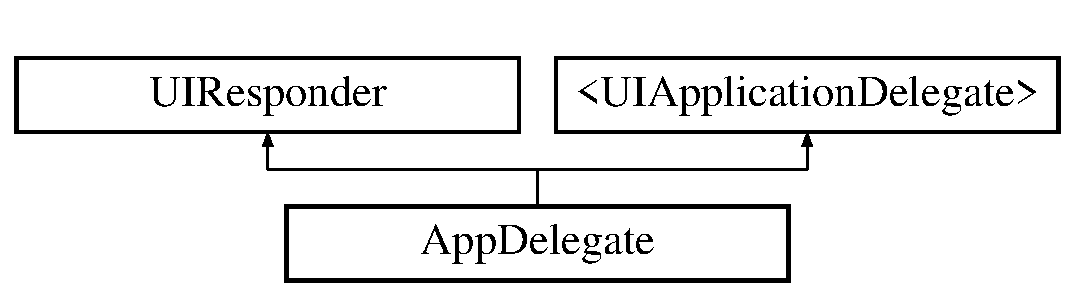
\includegraphics[height=2.000000cm]{interface_app_delegate}
\end{center}
\end{figure}
\subsection*{Properties}
\begin{DoxyCompactItemize}
\item 
\hypertarget{interface_app_delegate_acf48ac24125e688cac1a85445cd7fac2}{U\-I\-Window $\ast$ {\bfseries window}}\label{interface_app_delegate_acf48ac24125e688cac1a85445cd7fac2}

\item 
\hypertarget{interface_app_delegate_a89c5d4b85fcf7746042e1e1a67110d96}{\hyperlink{interface_login_view_controller}{Login\-View\-Controller} $\ast$ {\bfseries login\-View\-Controller}}\label{interface_app_delegate_a89c5d4b85fcf7746042e1e1a67110d96}

\end{DoxyCompactItemize}


The documentation for this class was generated from the following file\-:\begin{DoxyCompactItemize}
\item 
privly-\/ios/App\-Delegate.\-h\end{DoxyCompactItemize}

\hypertarget{interface_application_type_view_controller}{\section{Application\-Type\-View\-Controller Class Reference}
\label{interface_application_type_view_controller}\index{Application\-Type\-View\-Controller@{Application\-Type\-View\-Controller}}
}
Inheritance diagram for Application\-Type\-View\-Controller\-:\begin{figure}[H]
\begin{center}
\leavevmode
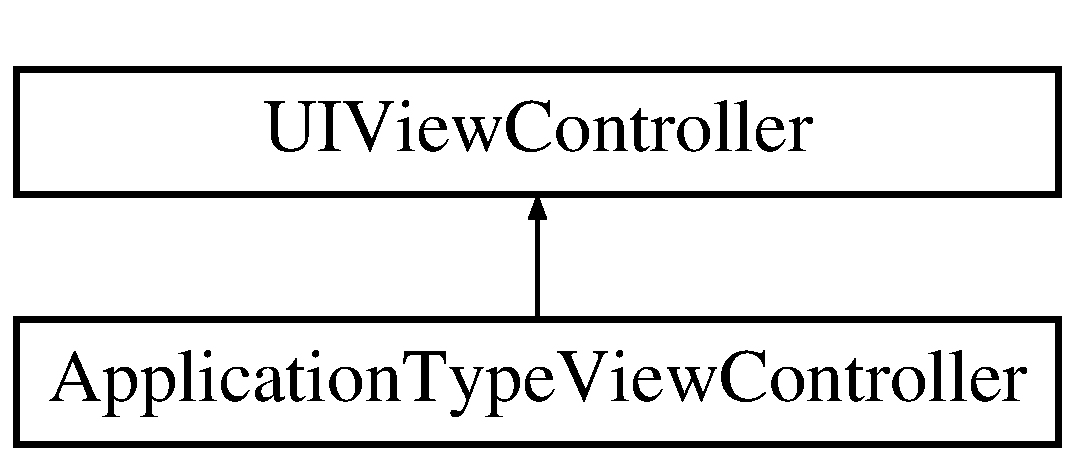
\includegraphics[height=2.000000cm]{interface_application_type_view_controller}
\end{center}
\end{figure}
\subsection*{Instance Methods}
\begin{DoxyCompactItemize}
\item 
\hypertarget{interface_application_type_view_controller_a9d9b997a57bb60fb2b52ec5014aad7c5}{(I\-B\-Action) -\/ {\bfseries create\-Plain\-Post\-:}}\label{interface_application_type_view_controller_a9d9b997a57bb60fb2b52ec5014aad7c5}

\item 
\hypertarget{interface_application_type_view_controller_a0f601aea82d2c60b2180a9846bad2426}{(I\-B\-Action) -\/ {\bfseries create\-Zero\-Bin\-Post\-:}}\label{interface_application_type_view_controller_a0f601aea82d2c60b2180a9846bad2426}

\item 
\hypertarget{interface_application_type_view_controller_adbdb011a5af34dcb65bbc0c7204d7f87}{(I\-B\-Action) -\/ {\bfseries create\-Test\-Post\-:}}\label{interface_application_type_view_controller_adbdb011a5af34dcb65bbc0c7204d7f87}

\item 
\hypertarget{interface_application_type_view_controller_a713c8146614cb2cba9b3dc3482ca7992}{(I\-B\-Action) -\/ {\bfseries logout\-:}}\label{interface_application_type_view_controller_a713c8146614cb2cba9b3dc3482ca7992}

\end{DoxyCompactItemize}


The documentation for this class was generated from the following files\-:\begin{DoxyCompactItemize}
\item 
privly-\/ios/Application\-Type\-View\-Controller.\-h\item 
privly-\/ios/Application\-Type\-View\-Controller.\-m\end{DoxyCompactItemize}

\hypertarget{category_application_type_view_controller_07_08}{\section{Application\-Type\-View\-Controller() Category Reference}
\label{category_application_type_view_controller_07_08}\index{Application\-Type\-View\-Controller()@{Application\-Type\-View\-Controller()}}
}


The documentation for this category was generated from the following file\-:\begin{DoxyCompactItemize}
\item 
privly-\/ios/Application\-Type\-View\-Controller.\-m\end{DoxyCompactItemize}

\hypertarget{interface_login_view_controller}{\section{Login\-View\-Controller Class Reference}
\label{interface_login_view_controller}\index{Login\-View\-Controller@{Login\-View\-Controller}}
}


View controller that handles user authentication.  




{\ttfamily \#import $<$Login\-View\-Controller.\-h$>$}

Inheritance diagram for Login\-View\-Controller\-:\begin{figure}[H]
\begin{center}
\leavevmode
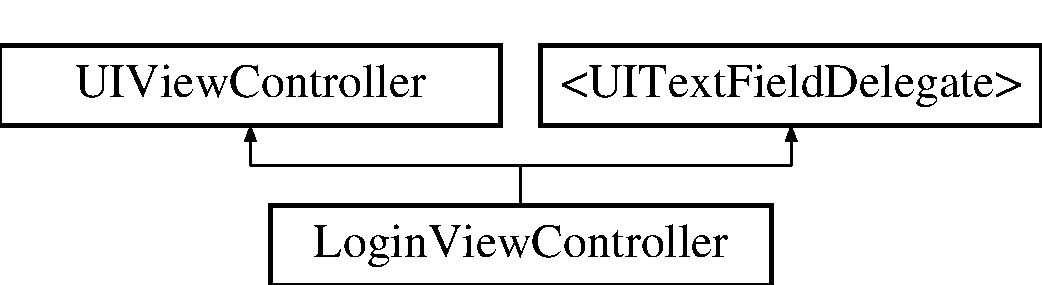
\includegraphics[height=2.000000cm]{interface_login_view_controller}
\end{center}
\end{figure}
\subsection*{Instance Methods}
\begin{DoxyCompactItemize}
\item 
(I\-B\-Action) -\/ \hyperlink{interface_login_view_controller_a89bdb3a2df5907f5902ddc31f1cdcf10}{get\-Token\-:}
\begin{DoxyCompactList}\small\item\em Parses username and password and fire authentication request. \end{DoxyCompactList}\end{DoxyCompactItemize}
\subsection*{Properties}
\begin{DoxyCompactItemize}
\item 
\hypertarget{interface_login_view_controller_a36c381bb3ebafaea2ae580c9c1b8f5b4}{I\-B\-Outlet U\-I\-Text\-Field $\ast$ \hyperlink{interface_login_view_controller_a36c381bb3ebafaea2ae580c9c1b8f5b4}{email\-Text\-Field}}\label{interface_login_view_controller_a36c381bb3ebafaea2ae580c9c1b8f5b4}

\begin{DoxyCompactList}\small\item\em Outlet for user email address textfield. \end{DoxyCompactList}\item 
\hypertarget{interface_login_view_controller_a88559585bce650e75448c94bf2619e33}{I\-B\-Outlet U\-I\-Text\-Field $\ast$ \hyperlink{interface_login_view_controller_a88559585bce650e75448c94bf2619e33}{password\-Text\-Field}}\label{interface_login_view_controller_a88559585bce650e75448c94bf2619e33}

\begin{DoxyCompactList}\small\item\em Outlet for user password textfield. \end{DoxyCompactList}\end{DoxyCompactItemize}


\subsection{Detailed Description}
View controller that handles user authentication. 

\subsection{Method Documentation}
\hypertarget{interface_login_view_controller_a89bdb3a2df5907f5902ddc31f1cdcf10}{\index{Login\-View\-Controller@{Login\-View\-Controller}!get\-Token\-:@{get\-Token\-:}}
\index{get\-Token\-:@{get\-Token\-:}!LoginViewController@{Login\-View\-Controller}}
\subsubsection[{get\-Token\-:}]{\setlength{\rightskip}{0pt plus 5cm}-\/ (I\-B\-Action) get\-Token\-: 
\begin{DoxyParamCaption}
\item[{(id)}]{sender}
\end{DoxyParamCaption}
}}\label{interface_login_view_controller_a89bdb3a2df5907f5902ddc31f1cdcf10}


Parses username and password and fire authentication request. 

\begin{DoxyReturn}{Returns}
Stores authentication token in N\-S\-User\-Defaults and returns 
\end{DoxyReturn}


The documentation for this class was generated from the following files\-:\begin{DoxyCompactItemize}
\item 
privly-\/ios/Login\-View\-Controller.\-h\item 
privly-\/ios/Login\-View\-Controller.\-m\end{DoxyCompactItemize}

\hypertarget{category_login_view_controller_07_08}{\section{Login\-View\-Controller() Category Reference}
\label{category_login_view_controller_07_08}\index{Login\-View\-Controller()@{Login\-View\-Controller()}}
}


The documentation for this category was generated from the following file\-:\begin{DoxyCompactItemize}
\item 
privly-\/ios/Login\-View\-Controller.\-m\end{DoxyCompactItemize}

\hypertarget{interface_plain_post_destination_view_controller}{\section{Plain\-Post\-Destination\-View\-Controller Class Reference}
\label{interface_plain_post_destination_view_controller}\index{Plain\-Post\-Destination\-View\-Controller@{Plain\-Post\-Destination\-View\-Controller}}
}
Inheritance diagram for Plain\-Post\-Destination\-View\-Controller\-:\begin{figure}[H]
\begin{center}
\leavevmode
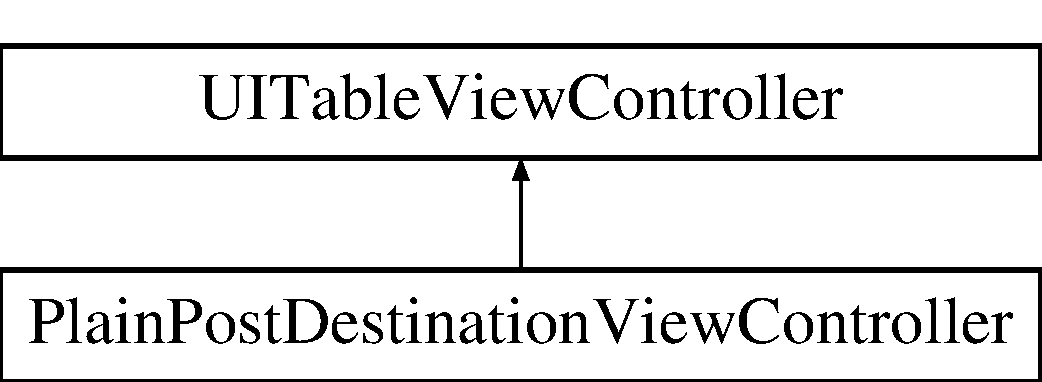
\includegraphics[height=2.000000cm]{interface_plain_post_destination_view_controller}
\end{center}
\end{figure}
\subsection*{Protected Attributes}
\begin{DoxyCompactItemize}
\item 
\hypertarget{interface_plain_post_destination_view_controller_a5933519d4d9ac6a4618a090a0ffba1b6}{N\-S\-Array $\ast$ {\bfseries available\-Services}}\label{interface_plain_post_destination_view_controller_a5933519d4d9ac6a4618a090a0ffba1b6}

\end{DoxyCompactItemize}


The documentation for this class was generated from the following file\-:\begin{DoxyCompactItemize}
\item 
privly-\/ios/Plain\-Post\-Destination\-View\-Controller.\-h\end{DoxyCompactItemize}

\hypertarget{category_plain_post_destination_view_controller_07_08}{\section{Plain\-Post\-Destination\-View\-Controller() Category Reference}
\label{category_plain_post_destination_view_controller_07_08}\index{Plain\-Post\-Destination\-View\-Controller()@{Plain\-Post\-Destination\-View\-Controller()}}
}


The documentation for this category was generated from the following file\-:\begin{DoxyCompactItemize}
\item 
privly-\/ios/Plain\-Post\-Destination\-View\-Controller.\-m\end{DoxyCompactItemize}

\hypertarget{interface_plain_post_view_controller}{\section{Plain\-Post\-View\-Controller Class Reference}
\label{interface_plain_post_view_controller}\index{Plain\-Post\-View\-Controller@{Plain\-Post\-View\-Controller}}
}
Inheritance diagram for Plain\-Post\-View\-Controller\-:\begin{figure}[H]
\begin{center}
\leavevmode
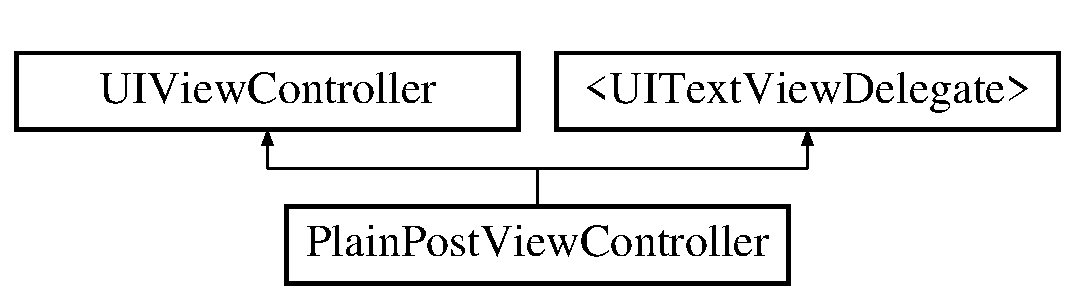
\includegraphics[height=2.000000cm]{interface_plain_post_view_controller}
\end{center}
\end{figure}
\subsection*{Instance Methods}
\begin{DoxyCompactItemize}
\item 
\hypertarget{interface_plain_post_view_controller_a9e60d5caeef9ee119c497cb5d890b7fd}{(I\-B\-Action) -\/ {\bfseries create\-Plain\-Post\-:}}\label{interface_plain_post_view_controller_a9e60d5caeef9ee119c497cb5d890b7fd}

\end{DoxyCompactItemize}
\subsection*{Properties}
\begin{DoxyCompactItemize}
\item 
\hypertarget{interface_plain_post_view_controller_af5675e8c08824561513ce64fc9620a5a}{I\-B\-Outlet U\-I\-Text\-View $\ast$ {\bfseries Plain\-Post\-Content}}\label{interface_plain_post_view_controller_af5675e8c08824561513ce64fc9620a5a}

\item 
\hypertarget{interface_plain_post_view_controller_a6c6d666c2655c0a8ff81f46debfabea6}{U\-I\-Bar\-Button\-Item $\ast$ {\bfseries dismiss\-Keyboard\-Button}}\label{interface_plain_post_view_controller_a6c6d666c2655c0a8ff81f46debfabea6}

\item 
\hypertarget{interface_plain_post_view_controller_a77f64c31823a1aa2e94a6ec3c841b06c}{int {\bfseries social\-Network\-Id}}\label{interface_plain_post_view_controller_a77f64c31823a1aa2e94a6ec3c841b06c}

\end{DoxyCompactItemize}


The documentation for this class was generated from the following files\-:\begin{DoxyCompactItemize}
\item 
privly-\/ios/Plain\-Post\-View\-Controller.\-h\item 
privly-\/ios/Plain\-Post\-View\-Controller.\-m\end{DoxyCompactItemize}

\hypertarget{category_plain_post_view_controller_07_08}{\section{Plain\-Post\-View\-Controller() Category Reference}
\label{category_plain_post_view_controller_07_08}\index{Plain\-Post\-View\-Controller()@{Plain\-Post\-View\-Controller()}}
}


The documentation for this category was generated from the following file\-:\begin{DoxyCompactItemize}
\item 
privly-\/ios/Plain\-Post\-View\-Controller.\-m\end{DoxyCompactItemize}

\hypertarget{interfaceprivly__ios__tests}{\section{privly\-\_\-ios\-\_\-tests Class Reference}
\label{interfaceprivly__ios__tests}\index{privly\-\_\-ios\-\_\-tests@{privly\-\_\-ios\-\_\-tests}}
}
Inheritance diagram for privly\-\_\-ios\-\_\-tests\-:\begin{figure}[H]
\begin{center}
\leavevmode
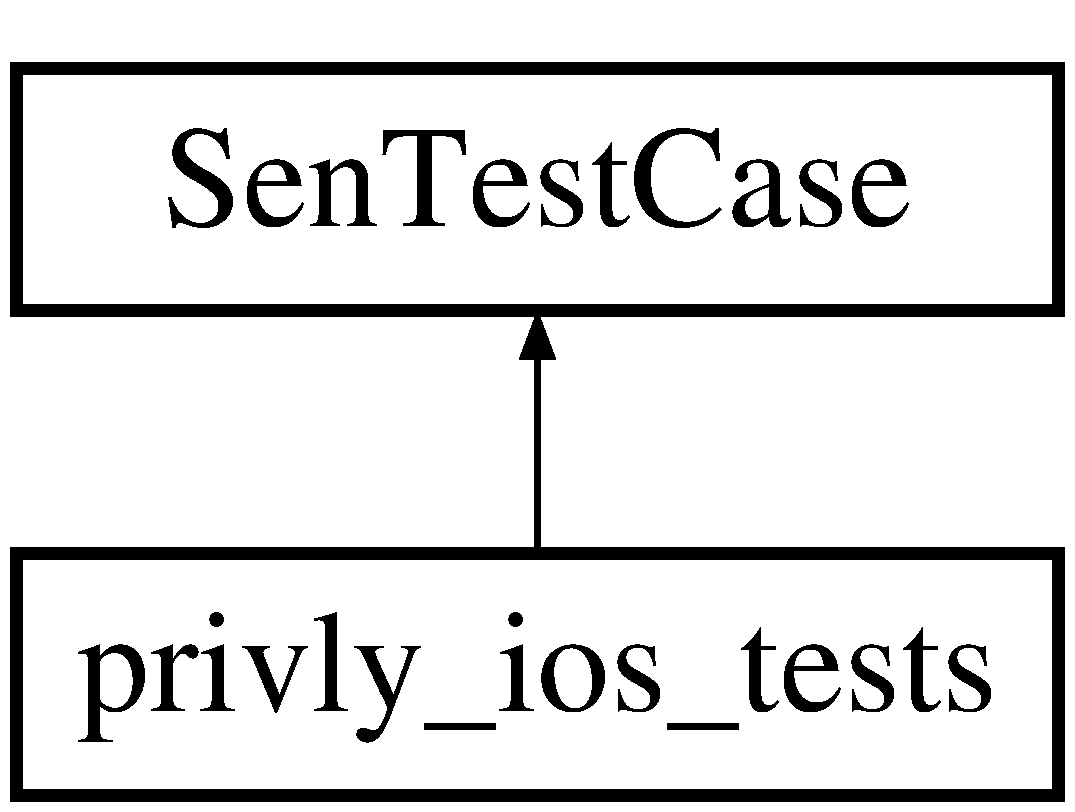
\includegraphics[height=2.000000cm]{interfaceprivly__ios__tests}
\end{center}
\end{figure}
\subsection*{Protected Attributes}
\begin{DoxyCompactItemize}
\item 
\hypertarget{interfaceprivly__ios__tests_af5c0c0653632470cbfe1b2a2df0b615c}{\hyperlink{interface_app_delegate}{App\-Delegate} $\ast$ {\bfseries app\-Delegate}}\label{interfaceprivly__ios__tests_af5c0c0653632470cbfe1b2a2df0b615c}

\item 
\hypertarget{interfaceprivly__ios__tests_af341988e0fa810104a5d968183663212}{\hyperlink{interface_login_view_controller}{Login\-View\-Controller} $\ast$ {\bfseries login\-View\-Controller}}\label{interfaceprivly__ios__tests_af341988e0fa810104a5d968183663212}

\end{DoxyCompactItemize}


The documentation for this class was generated from the following file\-:\begin{DoxyCompactItemize}
\item 
privly-\/ios-\/tests/privly\-\_\-ios\-\_\-tests.\-h\end{DoxyCompactItemize}

\hypertarget{interface_social_networks_request}{\section{Social\-Networks\-Request Class Reference}
\label{interface_social_networks_request}\index{Social\-Networks\-Request@{Social\-Networks\-Request}}
}
Inheritance diagram for Social\-Networks\-Request\-:\begin{figure}[H]
\begin{center}
\leavevmode
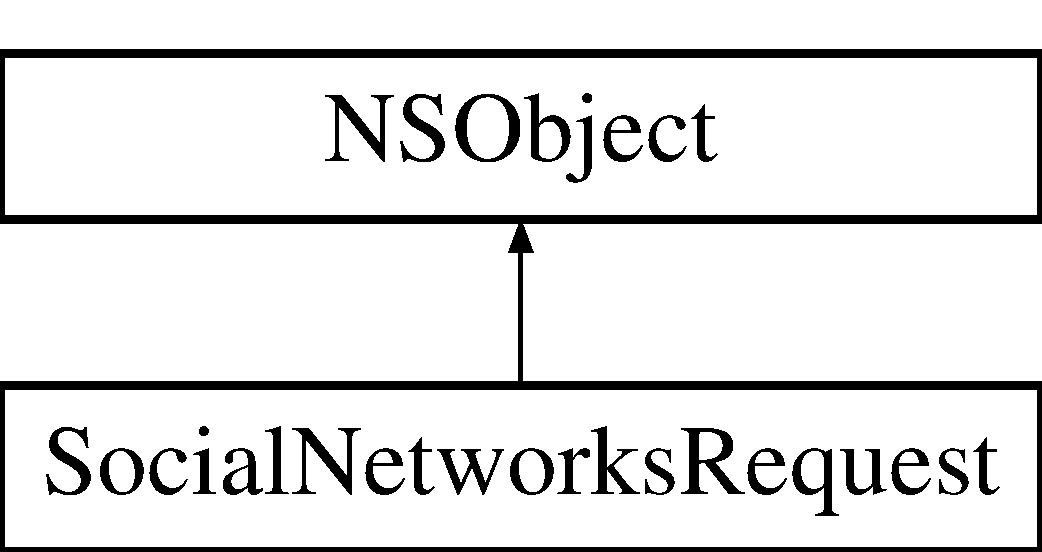
\includegraphics[height=2.000000cm]{interface_social_networks_request}
\end{center}
\end{figure}
\subsection*{Instance Methods}
\begin{DoxyCompactItemize}
\item 
\hypertarget{interface_social_networks_request_ab6682f7cab2530d12a34bbe1e59c9843}{(void) -\/ {\bfseries setup\-Account\-For\-Service\-Type\-Int\-:}}\label{interface_social_networks_request_ab6682f7cab2530d12a34bbe1e59c9843}

\item 
\hypertarget{interface_social_networks_request_abe9c76f079552368c2fb2bb4a7434b8f}{(void) -\/ {\bfseries post\-Message}}\label{interface_social_networks_request_abe9c76f079552368c2fb2bb4a7434b8f}

\end{DoxyCompactItemize}
\subsection*{Protected Attributes}
\begin{DoxyCompactItemize}
\item 
\hypertarget{interface_social_networks_request_a4ad54c11c8cb95cf5a0e343eff86d7a5}{N\-S\-String $\ast$ {\bfseries service\-Type\-String}}\label{interface_social_networks_request_a4ad54c11c8cb95cf5a0e343eff86d7a5}

\item 
\hypertarget{interface_social_networks_request_ad36e03b0ccaf96eff9a627075af99784}{N\-S\-String $\ast$ {\bfseries account\-Identifier\-String}}\label{interface_social_networks_request_ad36e03b0ccaf96eff9a627075af99784}

\end{DoxyCompactItemize}
\subsection*{Properties}
\begin{DoxyCompactItemize}
\item 
\hypertarget{interface_social_networks_request_a143e27a5d575ab752c8a00b39658f9ab}{U\-I\-View\-Controller $\ast$ {\bfseries delegate}}\label{interface_social_networks_request_a143e27a5d575ab752c8a00b39658f9ab}

\item 
\hypertarget{interface_social_networks_request_a4a1f36dc605e2f07a3185f70e22bb60a}{N\-S\-String $\ast$ {\bfseries post\-Content}}\label{interface_social_networks_request_a4a1f36dc605e2f07a3185f70e22bb60a}

\end{DoxyCompactItemize}


The documentation for this class was generated from the following files\-:\begin{DoxyCompactItemize}
\item 
privly-\/ios/Social\-Networks\-Request.\-h\item 
privly-\/ios/Social\-Networks\-Request.\-m\end{DoxyCompactItemize}

\hypertarget{interface_test_post_view_controller}{\section{Test\-Post\-View\-Controller Class Reference}
\label{interface_test_post_view_controller}\index{Test\-Post\-View\-Controller@{Test\-Post\-View\-Controller}}
}
Inheritance diagram for Test\-Post\-View\-Controller\-:\begin{figure}[H]
\begin{center}
\leavevmode
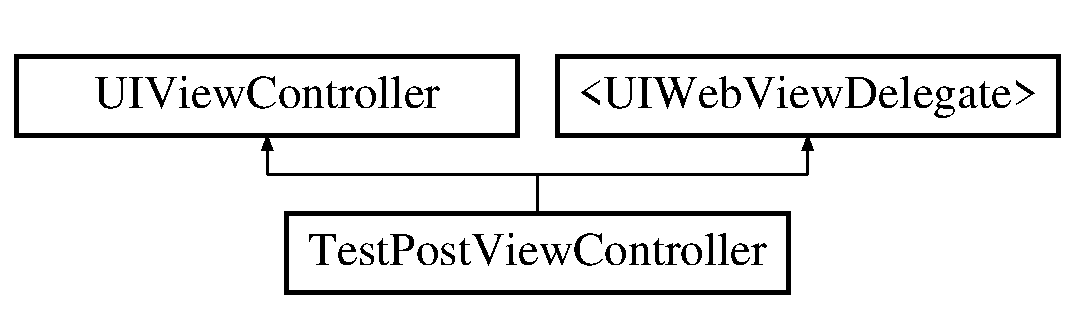
\includegraphics[height=2.000000cm]{interface_test_post_view_controller}
\end{center}
\end{figure}
\subsection*{Instance Methods}
\begin{DoxyCompactItemize}
\item 
\hypertarget{interface_test_post_view_controller_a771b1fa45892dd8f4f4a9ddffe5baa15}{(I\-B\-Action) -\/ {\bfseries load\-That\-J\-S\-:}}\label{interface_test_post_view_controller_a771b1fa45892dd8f4f4a9ddffe5baa15}

\end{DoxyCompactItemize}
\subsection*{Properties}
\begin{DoxyCompactItemize}
\item 
\hypertarget{interface_test_post_view_controller_a7428b142997a44872280c1e1443b44b8}{I\-B\-Outlet U\-I\-Web\-View $\ast$ {\bfseries test\-Post\-Web\-View}}\label{interface_test_post_view_controller_a7428b142997a44872280c1e1443b44b8}

\end{DoxyCompactItemize}


The documentation for this class was generated from the following files\-:\begin{DoxyCompactItemize}
\item 
privly-\/ios/Test\-Post\-View\-Controller.\-h\item 
privly-\/ios/Test\-Post\-View\-Controller.\-m\end{DoxyCompactItemize}

\hypertarget{category_test_post_view_controller_07_08}{\section{Test\-Post\-View\-Controller() Category Reference}
\label{category_test_post_view_controller_07_08}\index{Test\-Post\-View\-Controller()@{Test\-Post\-View\-Controller()}}
}


The documentation for this category was generated from the following file\-:\begin{DoxyCompactItemize}
\item 
privly-\/ios/Test\-Post\-View\-Controller.\-m\end{DoxyCompactItemize}

\hypertarget{interface_zero_bin_post_view_controller}{\section{Zero\-Bin\-Post\-View\-Controller Class Reference}
\label{interface_zero_bin_post_view_controller}\index{Zero\-Bin\-Post\-View\-Controller@{Zero\-Bin\-Post\-View\-Controller}}
}
Inheritance diagram for Zero\-Bin\-Post\-View\-Controller\-:\begin{figure}[H]
\begin{center}
\leavevmode
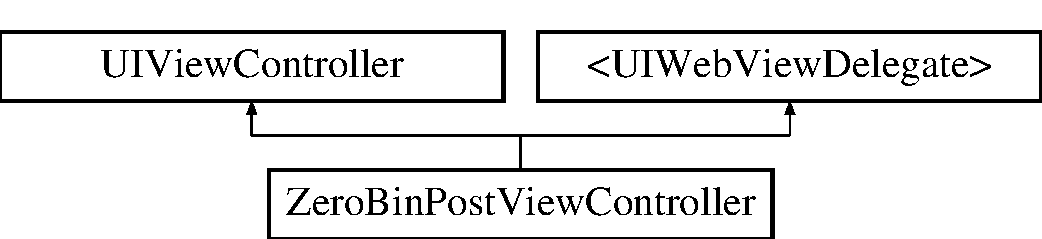
\includegraphics[height=2.000000cm]{interface_zero_bin_post_view_controller}
\end{center}
\end{figure}
\subsection*{Properties}
\begin{DoxyCompactItemize}
\item 
\hypertarget{interface_zero_bin_post_view_controller_abe2e097f9dd6ecb3758d8d0698da1377}{I\-B\-Outlet U\-I\-Web\-View $\ast$ {\bfseries zero\-Bin\-Web\-View}}\label{interface_zero_bin_post_view_controller_abe2e097f9dd6ecb3758d8d0698da1377}

\end{DoxyCompactItemize}


The documentation for this class was generated from the following file\-:\begin{DoxyCompactItemize}
\item 
privly-\/ios/Zero\-Bin\-Post\-View\-Controller.\-h\end{DoxyCompactItemize}

\hypertarget{category_zero_bin_post_view_controller_07_08}{\section{Zero\-Bin\-Post\-View\-Controller() Category Reference}
\label{category_zero_bin_post_view_controller_07_08}\index{Zero\-Bin\-Post\-View\-Controller()@{Zero\-Bin\-Post\-View\-Controller()}}
}


The documentation for this category was generated from the following file\-:\begin{DoxyCompactItemize}
\item 
privly-\/ios/Zero\-Bin\-Post\-View\-Controller.\-m\end{DoxyCompactItemize}

%--- End generated contents ---

% Index
\newpage
\phantomsection
\addcontentsline{toc}{part}{Index}
\printindex

\end{document}
